\vspace{1cm}
    \begin{figure}[thb!]
        \centering
        \begin{minipage}{0.8\textwidth}
           \captionsetup[sub]{font=small}
            \begin{minipage}[h!]{0.8\textwidth}
                \begin{subfigure}[b!]{0.44 \textwidth}
                    \caption{$\epsilon = 1\%$}
                    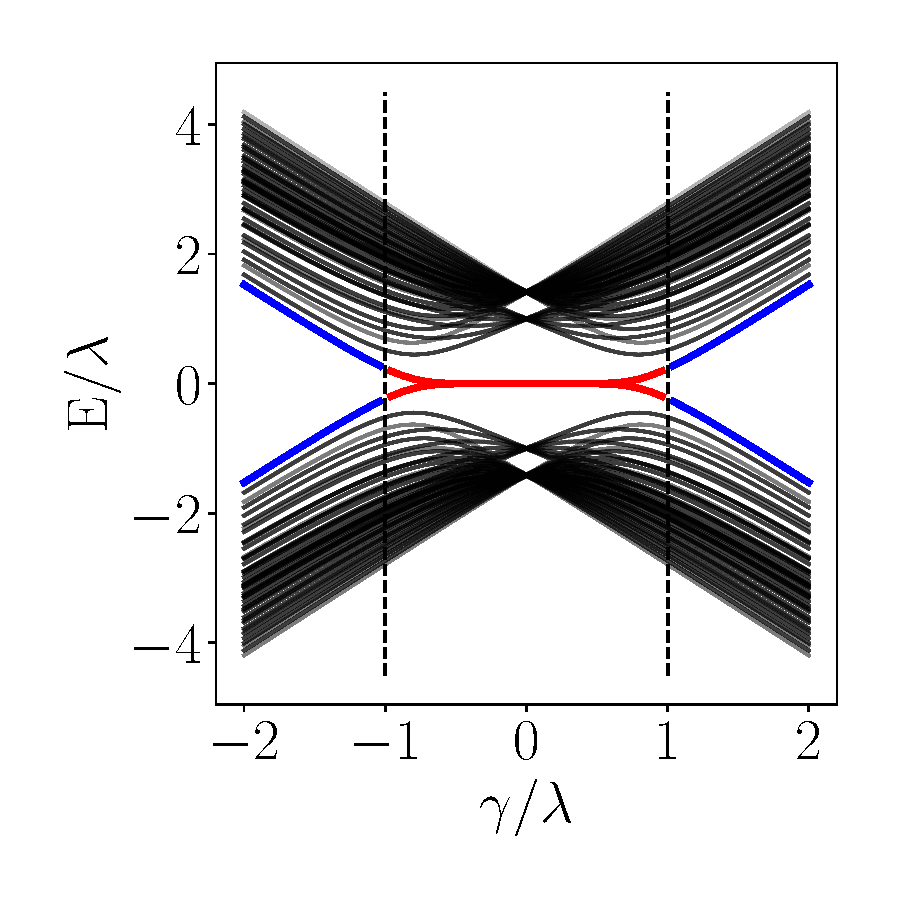
\includegraphics[width=\textwidth]{Imagenes/Resultados_Hoti_Cuadrado/bands_square_shh_0.01.pdf}
                \end{subfigure}\hspace*{-0.5em}
                \begin{subfigure}[b!]{0.56 \textwidth}
                    \caption*{}
                    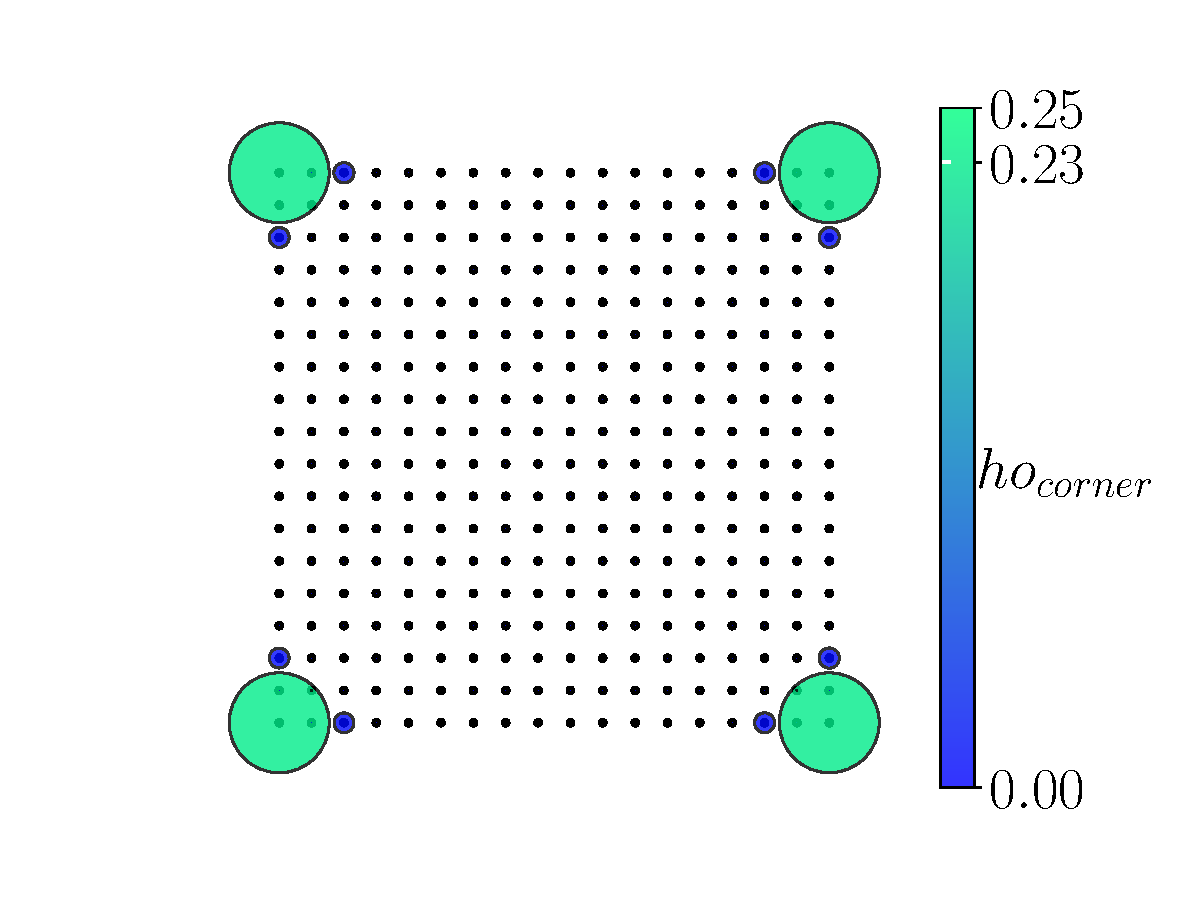
\includegraphics[width=\textwidth]{Imagenes/Resultados_Hoti_Cuadrado/proyection_square_0.01.pdf}
                \end{subfigure}\hspace*{-0.5em}
            \end{minipage}\vspace*{-1.5em}
            
            \begin{minipage}[h!]{0.8\textwidth}
                \begin{subfigure}[b!]{0.44 \textwidth}
                    \caption{$\epsilon = 5\%$}
                    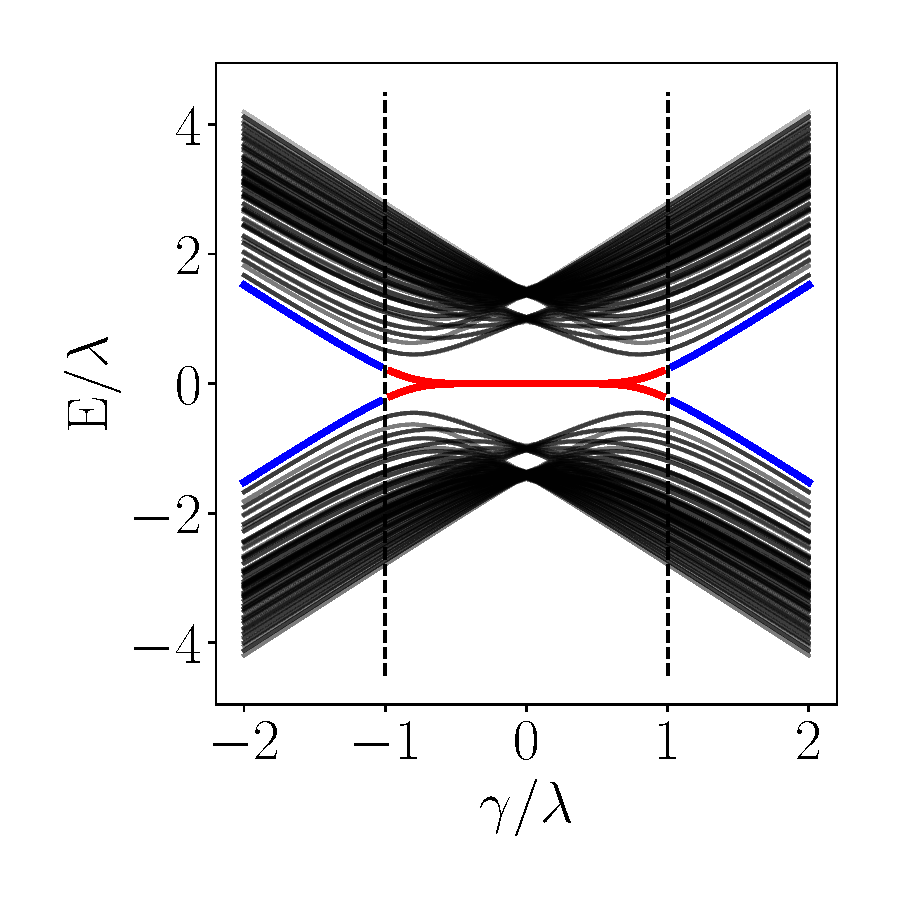
\includegraphics[width=\textwidth]{Imagenes/Resultados_Hoti_Cuadrado/bands_square_shh_0.05.pdf}
                \end{subfigure}\hspace*{-0.5em}
                \begin{subfigure}[b!]{0.56 \textwidth}
                    \caption*{}
                    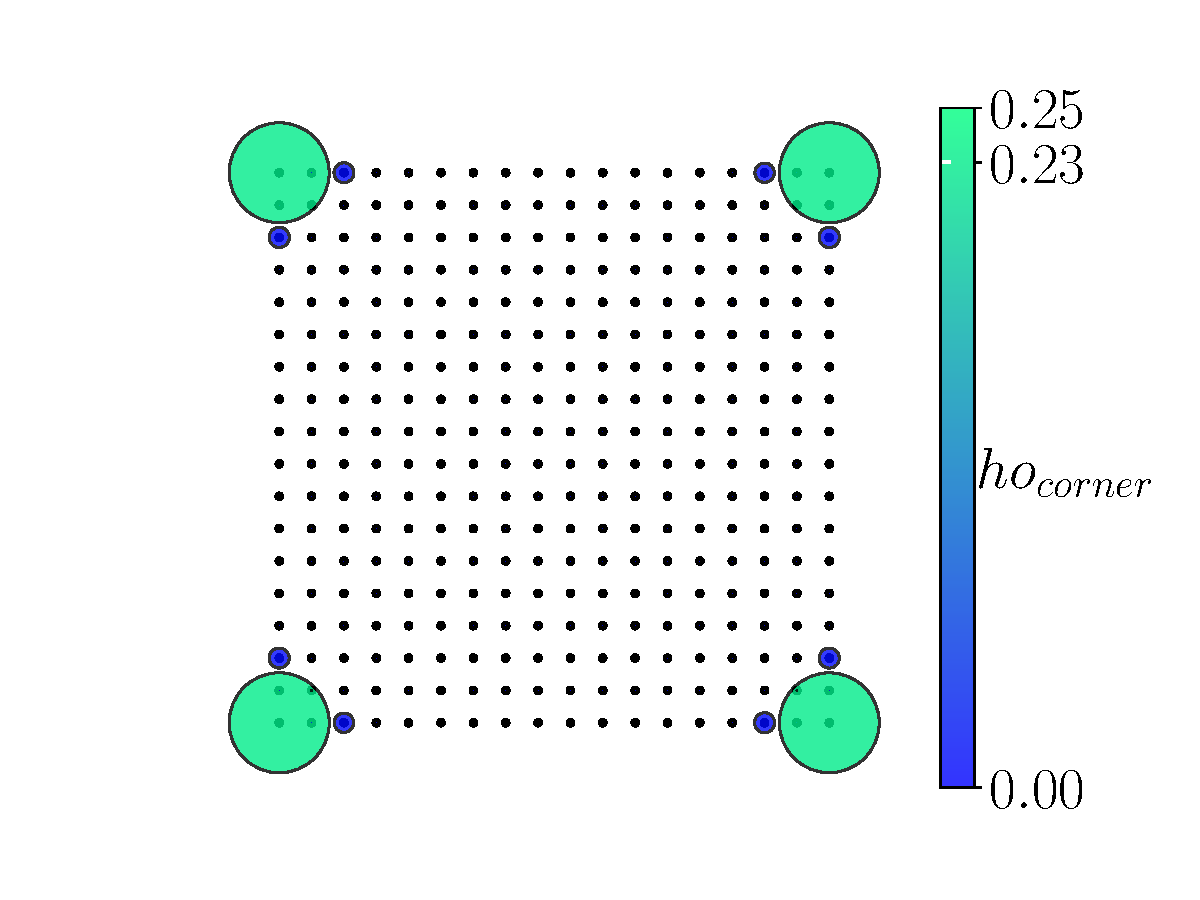
\includegraphics[width=\textwidth]{Imagenes/Resultados_Hoti_Cuadrado/proyection_square_0.05.pdf}
                \end{subfigure}\hspace*{-0.5em}
            \end{minipage}\vspace*{-1.5em}
            
            \begin{minipage}[h!]{0.8\textwidth}
                \begin{subfigure}[b!]{0.44 \textwidth}
                    \caption{$\epsilon = 10\%$}
                    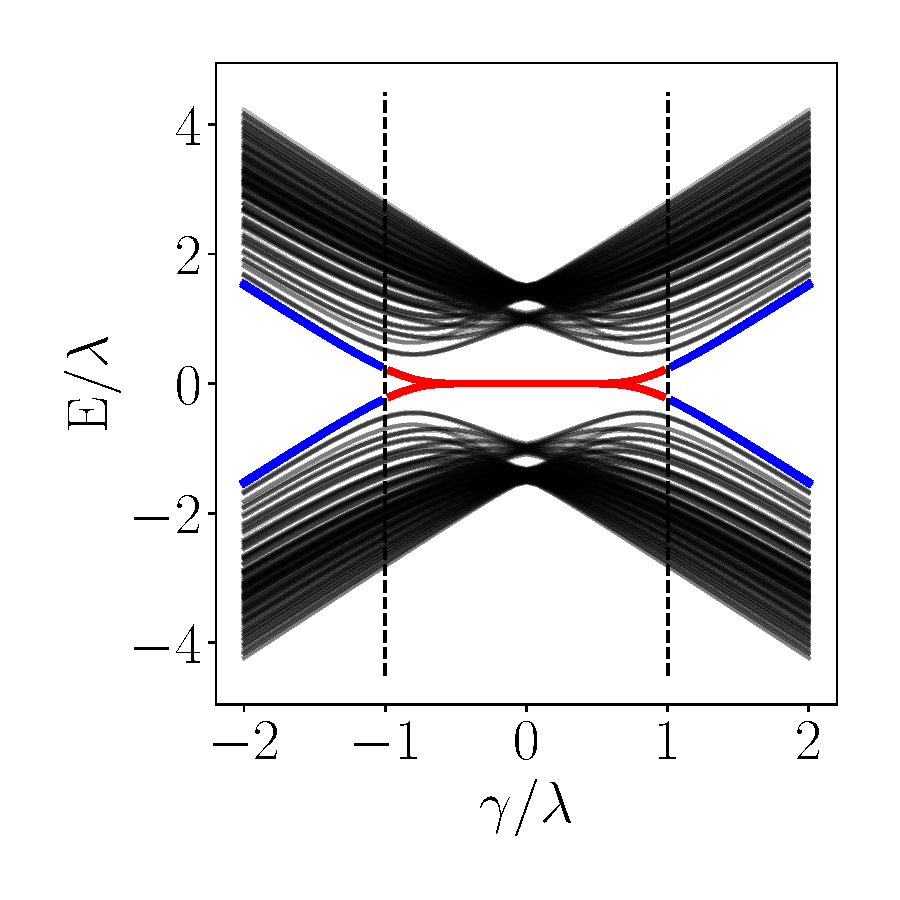
\includegraphics[width=\textwidth]{Imagenes/Resultados_Hoti_Cuadrado/bands_square_shh_0.1.pdf}
                \end{subfigure}\hspace*{-0.5em}
                \begin{subfigure}[b!]{0.56 \textwidth}
                    \caption*{}
                    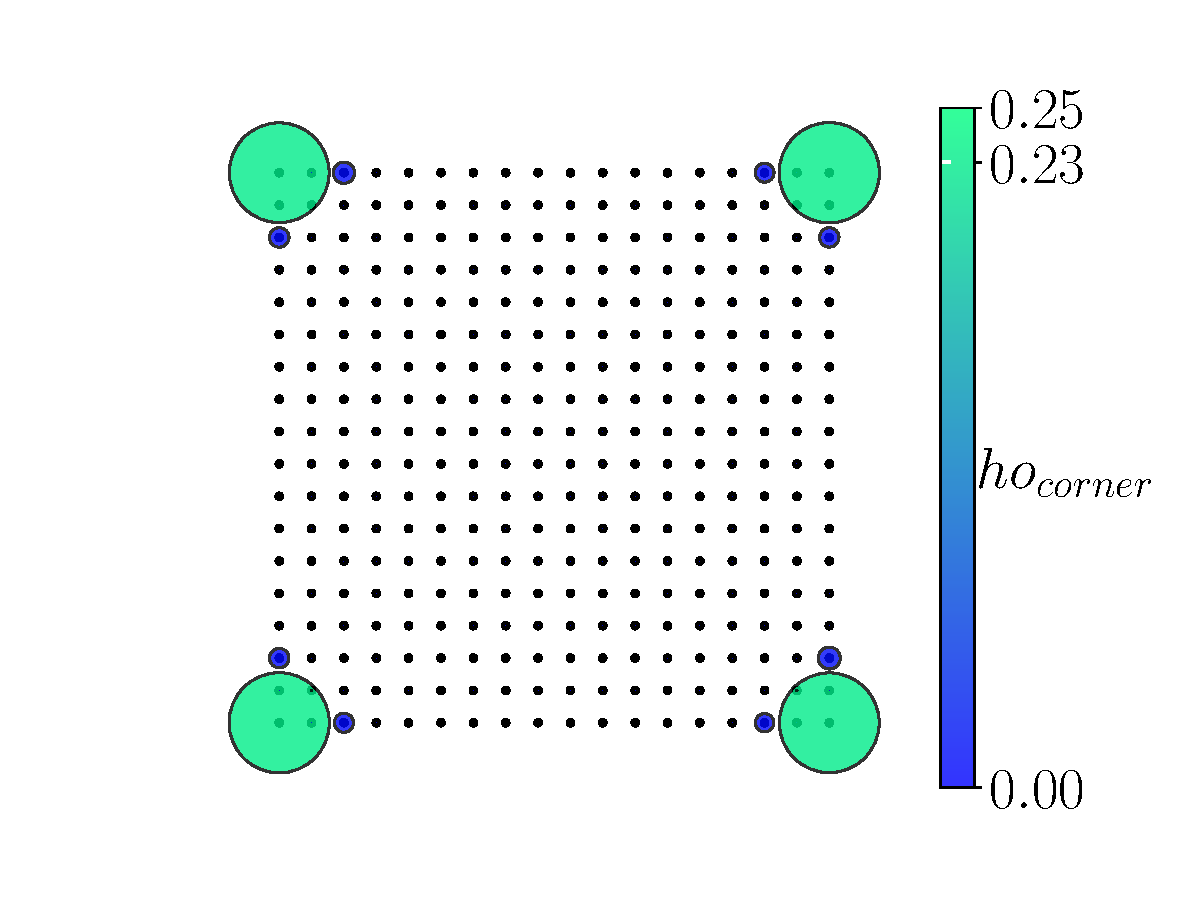
\includegraphics[width=\textwidth]{Imagenes/Resultados_Hoti_Cuadrado/proyection_square_0.1.pdf}
                \end{subfigure}\hspace*{-0.5em}
            \end{minipage}\vspace*{-1.5em}
            
            \begin{minipage}[h!]{0.8\textwidth}
                \begin{subfigure}[b!]{0.44 \textwidth}
                    \caption{$\epsilon = 30\%$}
                    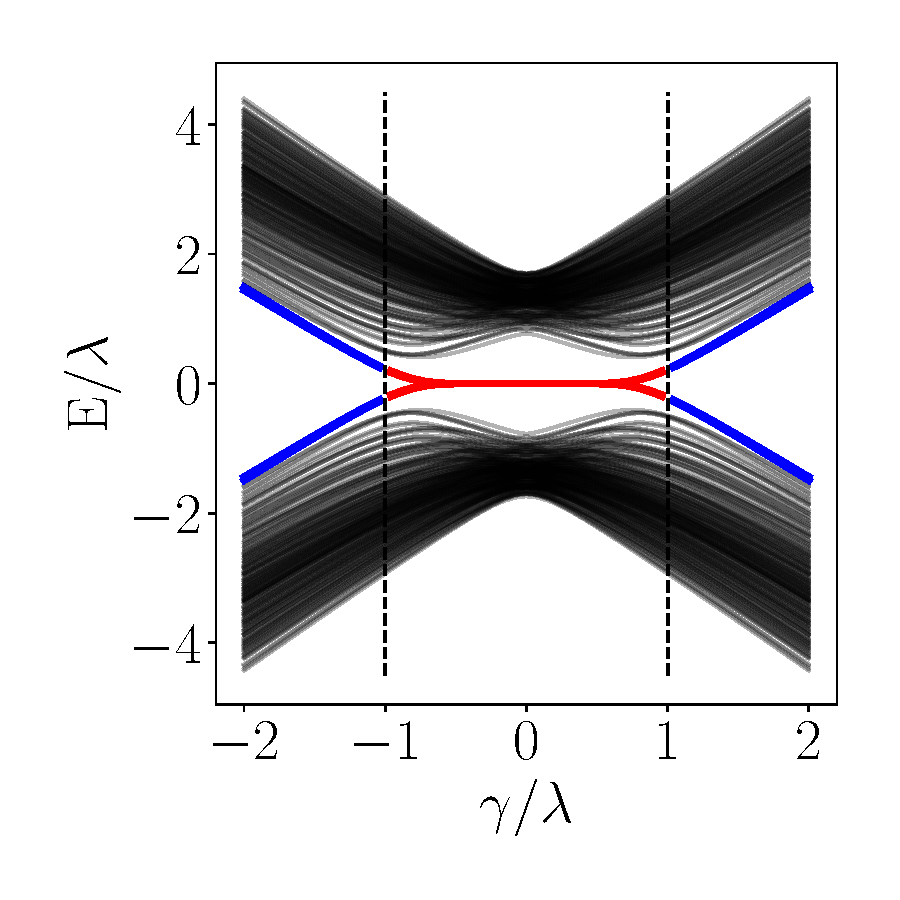
\includegraphics[width=\textwidth]{Imagenes/Resultados_Hoti_Cuadrado/bands_square_shh_0.3.pdf}
                \end{subfigure}\hspace*{-0.5em}
                \begin{subfigure}[b!]{0.56 \textwidth}
                    \caption*{}
                    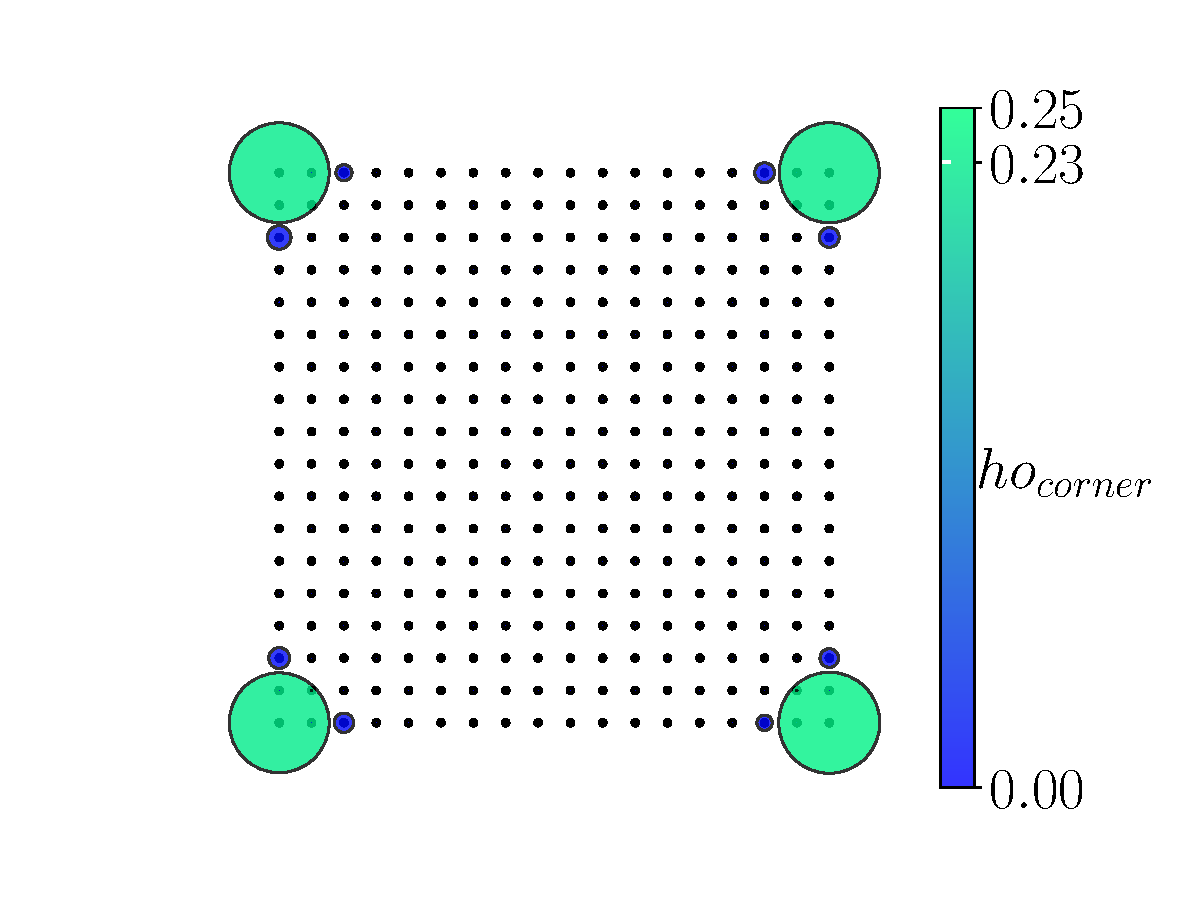
\includegraphics[width=\textwidth]{Imagenes/Resultados_Hoti_Cuadrado/proyection_square_0.3.pdf}
                \end{subfigure}\hspace*{-0.5em}
            \end{minipage}\vspace*{-1.5em}
            
            \begin{minipage}[h!]{0.8\textwidth}
                \begin{subfigure}[b!]{0.44 \textwidth}
                    \caption{$\epsilon = 50\%$}
                    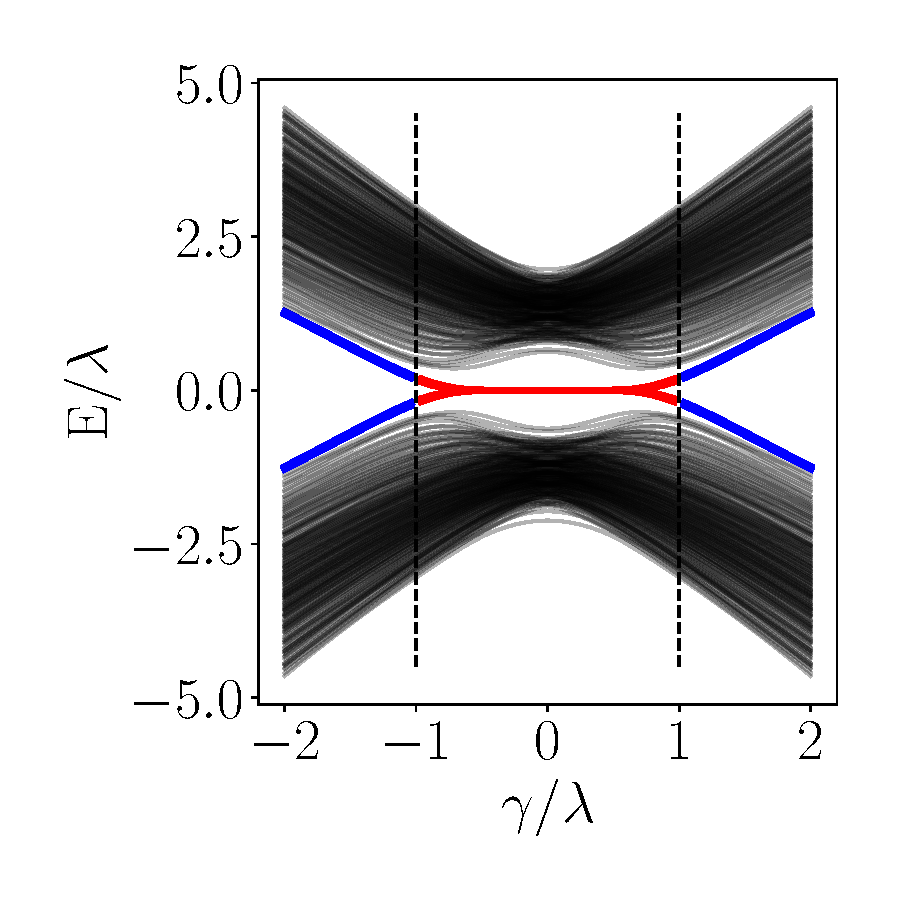
\includegraphics[width=\textwidth]{Imagenes/Resultados_Hoti_Cuadrado/bands_square_shh_0.5.pdf}
                \end{subfigure}\hspace*{-0.5em}
                \begin{subfigure}[b!]{0.56 \textwidth}
                    \caption*{}
                    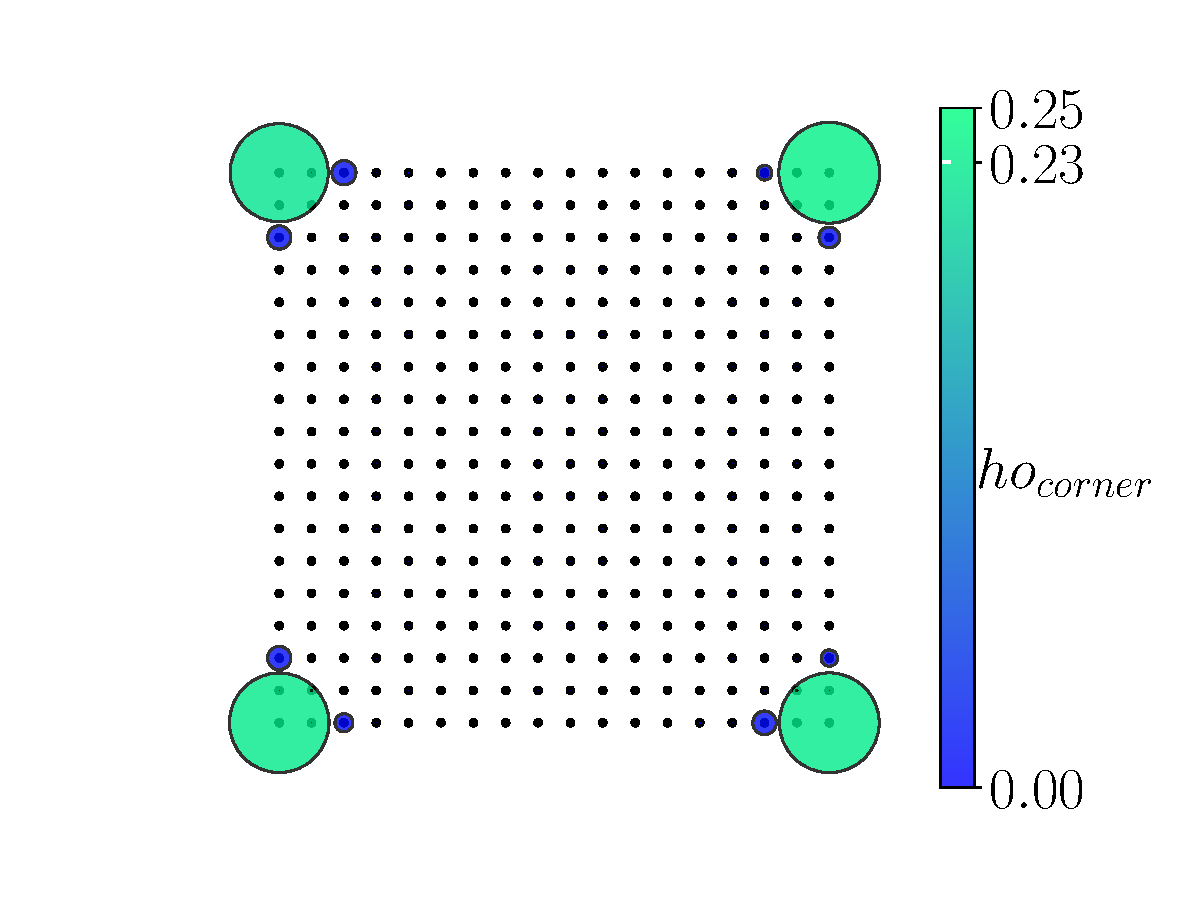
\includegraphics[width=\textwidth]{Imagenes/Resultados_Hoti_Cuadrado/proyection_square_0.5.pdf}
                \end{subfigure}\hspace*{-0.5em}
            \end{minipage}\vspace*{-0.5em}
        \end{minipage} 
           \caption{\textbf{(a)-(e)}En la columna derecha se muestra el espectro de energías en una red cuadrada como función de $\gamma/\lambda $ con un desorden aleatorio en los parámetros de salto, de tamaño $\delta$. Las lineas rojas corresponden a los cuatro estados degenerados que representan los estados localizados en las esquinas. En la columna izquierda se muestra la densidad de probabilidad de la fase no trivial donde $\gamma' = \gamma( 1 \pm \epsilon) ,\, \, \lambda' = \lambda( 1 \pm \epsilon)$.  }
           \label{fig:Pram_Proy_Delta_cuadrado}
         
       \end{figure} 

    

